\documentclass[10pt,a4paper]{article}
\usepackage[italian]{babel}
\usepackage{listings}
\usepackage{xcolor}
\usepackage{graphicx}
\usepackage{listings}
\usepackage{hyperref}

\graphicspath{{./}}

\definecolor{backgrey}{rgb}{0.92, 0.92, 0.92}

\lstdefinestyle{none}{
    basicstyle={\small\ttfamily},
    backgroundcolor=\color{backgrey}
}

\begin{document}

\begin{titlepage}
\end{titlepage}

\tableofcontents
\newpage

\section{Introduction - what is constraint programming?}
The combinatorial decision making is a generic problem where we have to make a
decision (obviously) within many cases of a context and with a number of
restrictions, usually called constraints. A solution can be any which meets all
constraints, but also an optimal solution according to an objective. This
problem is quite common in out daily lives, think about hospitals during covid:
infected people had to be assigned to hospitals according to some parameters
like the severity of illness, the age, the hospital resources. One can object
that this can be done with artificial intelligence, but this is very tricky,
because for this specific problem we have no data for training and, in general,
neural networks are very expensive to train, if we want something which have a
useful accuracy. Decision making is typically computationally difficult
(NP-hard) and there are many techniques to approach it: integer linear
programming; boolean SATisfiability; constraint programming. We will focus on
\textit{constraint programming} (CP). But what is constraint programming? It is
a declarative programming paradigm for expressing and solving combinatorial
optimization problems. These problems have to be expressed as a model which has
typically three entities:
\begin{itemize}
    \item the unknowns, namely decision variables which we have to find a value
    for;
    \item the possible values for the unknowns;
    \item relations between unknowns.
\end{itemize}
The power of CP stands in the solving, indeed, the user doesn't have to worry
about how it can solve a problem, but just how to model it. This is possible
thanks to the \textit{solver}, which, given a model for a problem, has the goal
of solving the problem, by assigning values to unknowns.

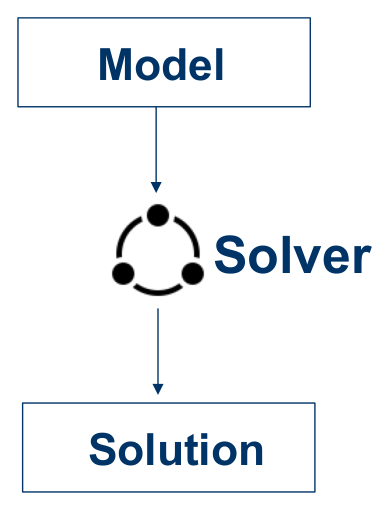
\includegraphics[scale=0.2]{solver.png}

But how does a solver work? It uses a backtracking tree search for guessing the
values for variables and it examines model constraints to shrink domains of
decision variables in order to avoid incompatible values in the future (this is
called \textit{propagation}). But these phases are separated, indeed, it
interleaves cycles of variables assigning and propagation. Modelling is
critical, since the solver depends on it.

\pagebreak

\section{Model}
Now, we can formalize the concepts
around CP. A constraint satisfaction problem (CSP) is a triple $ \langle X, D,
C \rangle $, where:
\begin{itemize}
    \item $X$ is a finite set of decision variables $X_1, ..., X_n$ which
    require a value to be assigned to;
    \item $D$ is the set of domains of $X$, so $X_i \in D_i(X_i)$; each $D_i$ is
    supposed to be finite;
    \item $C$ is a set of constraints, namely relations over the domains:
    \[ C_i \subseteq D_j(X_j) \times ... \times D_k(X_k) \]
\end{itemize}

A constraint optimization problem is 4-tuple $ \langle X, D, C, f \rangle $,
where $f$ is an objective variable whose value has to be optimized, namely
minimizing or maximizing it.

\subsection{Constraints}
There are two main kinds of constraints representations:
\begin{itemize}
    \item \textit{extensional} constraints which relies on the fact that any
    kind of constraint can be expressed as the set of all allowed combinations,
    for example $C(X_1, X_2) = {(0,0), (0,2), (1,3), (2,1)}$;
    \item \textit{intensional} constraints, namely declarative relations on
    involved entities, for example $X > Y$.
\end{itemize}

\paragraph{Channeling constraints}
Channeling constraints makes two different models ``comunicate", in the sense
that, given two models $m1$ and $m2$ and a channeling constraint $c$, $c$ brings
what has been discovered in $m1$ in $m2$ and viceversa thanks to different
propagation algorithms in different models $m1$ and $m2$. This improves
propagation because benefits from a model are brought to another model. Think
about n-queens problem where we have to place $n$ queens in a $n \times n$
chests board in order to they cannot eat directly any queen. We can have
different models for this problem.

First model:
\[ X_1, ..., X_n \in {1, ..., n} \]
\[ \textrm{alldifferent}([X_1, ..., X_n]) \]
\[ \textrm{alldifferent}([X_1 + 1, ..., X_n + n]) \]
\[ \textrm{alldifferent}([X_1 - 1, ..., X_n - n]) \]

\pagebreak

Second model:
\[ n \times n \; B_{ij} \in {0, 1} \]
\[ \sum_{i \in {1, ..., n}} B_{ij} = 1, \; \forall j \in {1, ..., n} \]
\[ \sum_{j \in {1, ..., n}} B_{ij} = 1, \; \forall i \in {1, ..., n} \]
\[ \sum B_{ij} \leq 1 \; \textrm{on all diagonals} \]
\[ \textrm{lex-lesser-eq}(B, \pi(B)), \; \forall \pi \]
The two models represent the same problem. The first one uses variables to
represent queens positions on the board and it exploits the alldifferent
constraint, while the second one uses a boolean matrix to represent the
positions and it exploits the lexicographic order constraint. They have
different benefits on search (not explained which benefits there, take this as
granted), so how to take advantage from both? We use a channeling constraint:

\[ \forall i, j \; X_i = j \iff B_{ij} = 1 \]

\paragraph{Meta-constraints}
A \textit{meta-constraint} is a constraint occurring in another constraint. For
example $ \sum_{i} (X_i > t_i) <= n $; in this case, the inner constraint is
$ (X_i > t_i) $. This type of constraints is useful when we want to make choices
according to the results of other constraints.

\paragraph{Implied and redundant constraints}
An \textit{implied constraint} is a semantically redundant and they speed up the
solver. On the other hand, we refer to redundant constraint as a constraint
which is semantically redundant, but it doesn't affect the solver performance.
It happens to have a redudant constraint $r$ when we have another constraint $s$
which makes the propagation shrink the domains of variables in the same way $r$
would do. For example, look at this model:

\begin{lstlisting}[style=none]
include "alldifferent.mzn";
int: n;
array [0..n-1] of var 0..n-1: x;

constraint forall(i in 0..n-1)
    (x[i] = sum (j in 0..n-1)(x[j] == i));

constraint sum(i in 0..n-1)(x[i]) = n;

constraint sum(i in 0..n-1)(x[i]*i) = n;

solve satisfy;
\end{lstlisting}

In this model, we are expressing the sequence puzzle problem, namely we want to
make a sequence $x$ with length $n$, where for each $i \in {1, ..., n}$, $i$
appears exactly $x_i$ times in the sequence $x$. Note that we don't used global
constraints. The last two constraints are implied, so they affect solver
performance. Now consider the following model:

\begin{lstlisting}[style=none]
include "globals.mzn";

int: n;
array [1..n] of var 0..n-1: x;

constraint let {
  array[1..n] of 0..n-1: cover = 0..n-1
} in global_cardinality(x, cover, x);

constraint sum(i in 1..n) (x[i]) = n;

constraint sum(i in 1..n) (x[i] * (i-1)) = n;

solve satisfy;
\end{lstlisting}
This model is semantically equivalent to the previous one, but the first implied
constraint (so the second constraint) became redundant. This happened because
the propagation algorithm for \texttt{global\_cardinality\_constraint} is more
effective than decomposition and so it ``discovers" all the first (ex-)implied
constraint would do. This concept will be developed better nextly.

\subsection{Symmetry}
Often, when we try to solve a problem, tehre are many solutions which are
``symmetric". Two solutions are symmetric if one of them is a permutation of the
other one. The solver cannot know if two solutions are symmetric and it will
look for all of them, but this is a waste of time because two symmetric
solutions are actually the same solution, they didn't bring something new. Thus,
to avoid symmetry, we can add some constraints which somehow impose an order in
order to accept just one solution and exclude all the symmetric ones. Usually,
useful constraints are the ones of \texttt{lex*} family, namely constraints
which pretend lexicographic order on array of variables.
TODO

\section{Constraints propagation}
Propagation is the action of restricting the domains of variables.

\subsection{Local consistency}
This is a form of inference which detects inconsistent partial assignments. What
is a partial assignment? An assignment is literally an assignment of a value to
a decision variable:

\[ X_i = j \]

If that assignment is inconsistent, then $j$ can be removed from $D(X_i)$ and,
as a consequence, it helps propagation.

\subsubsection{Generalized Arc Consistency}
A \textit{support} $(d_1, ..., d_k) \in (D(X_1), ..., D(X_k))$  for a constraint
$C$ is an assignment of decision variables which satisfies $C$.
A constraint $C$ is \textit{GAC} iff $\forall X_i \in {X_i, ..., X_n}$,
$\forall v \in D(X_i)$, $v \in d_i$, where $d_i$ is a support of $C$.
This is called \textit{Arc consistency} ($AC$) when $k = 2$.

In other words, a constraint $C$ restricts the domains $D(X_i)$. A question can
arise: how does a constraint $C$ grant the property of $GAC$ for domains? The
answer is that global constraints have specialized propagation algorithms. These
algorithms tries to keep the domains of variables as restricted as possible in
order to have always the lowest number assignments.

\subsubsection{Bounds consistency}
It relaxes the domain of a decision variable $X_i$ to be in a range such that

\[ D(X_i) = [min(X_i)...max(X_i)] \]

A \textit{bound support} is a tuple $(d_1, ..., d_k) \in C$ where
$d_i \in [min(X_i)...max(X_i)]$.

$C(X_i, ..., X_k)$ is BC iff for all $X_i \in {X_1, ..., X_k}$, $min(X_i)$ and
$max(X_i)$ belong to a bound support. GAC is stronger than BC, however, it's
more expensive to achieve sometimes.

Look at the following minizinc programs to solve sudoku:

\begin{lstlisting}[style=none]
include "globals.mzn";

int: n;

array[1..(n*n), 1..(n*n)] of var 1..(n*n): x;

% Rows must be all different
constraint forall(i in 1..(n*n)) (alldifferent(x[i, ..])
    ::domain_propagation
    );

% Columns must be all different
constraint forall(j in 1..(n*n)) (alldifferent(x[.., j])
    ::domain_propagation
    );

% Squares must be all different
constraint forall (i in 1..n) (forall (j in 1..n)
	(alldifferent(x[(1+((i-1)*n))..(n+((i-1)*n)),
                    (1+((j-1)*n))..(n+((j-1)*n))]))
                    ::domain_propagation
	);

solve satisfy;
\end{lstlisting}

and:

\begin{lstlisting}[style=none]
include "globals.mzn";

int: n;

array[1..(n*n), 1..(n*n)] of var 1..(n*n): x;

% Rows must be all different
constraint forall(i in 1..(n*n)) (alldifferent(x[i, ..])
    ::bounds_propagation
    );

% Columns must be all different
constraint forall(j in 1..(n*n)) (alldifferent(x[.., j])
    ::bounds_propagation
    );

% Squares must be all different
constraint forall (i in 1..n) (forall (j in 1..n)
	(alldifferent(x[(1+((i-1)*n))..(n+((i-1)*n)),
                    (1+((j-1)*n))..(n+((j-1)*n))]))
                    ::bounds_propagation
	);

solve satisfy;
\end{lstlisting}

and:

\begin{lstlisting}[style=none]
include "globals.mzn";

int: n;

array[1..(n*n), 1..(n*n)] of var 1..(n*n): x;

% Rows must be all different
constraint forall(i in 1..(n*n)) (alldifferent(x[i, ..]));

% Columns must be all different
constraint forall(j in 1..(n*n)) (alldifferent(x[.., j]));

% Squares must be all different
constraint forall (i in 1..n) (forall (j in 1..n)
	(alldifferent(x[(1+((i-1)*n))..(n+((i-1)*n)),
                    (1+((j-1)*n))..(n+((j-1)*n))]))
	);

solve satisfy;
\end{lstlisting}

We try to solve it with $n = 7$, so we are solving a sudoku 49X49. In the
first program, we specify (or better, we suggest) to use domain propagation,
namely we keep $GAC$. Results are these:

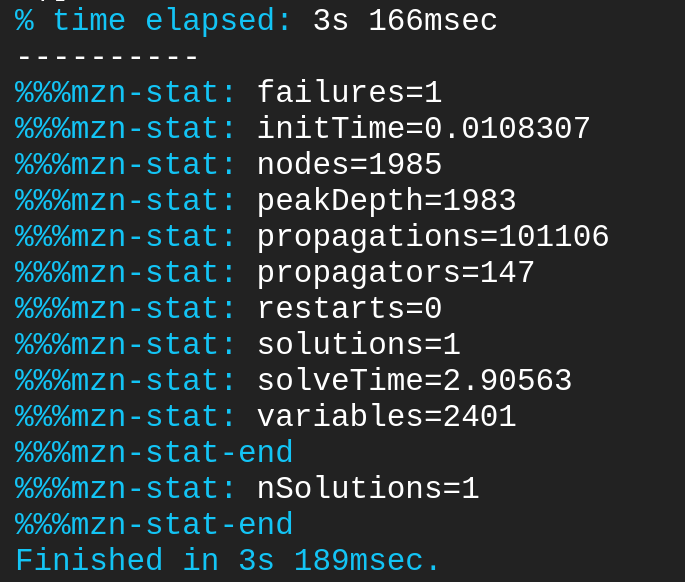
\includegraphics[scale=0.2]{sudoku_res.png}

Just 3 seconds, not bad! But when we try to use bounds propagation (namely $BC$)
or even not to suggest the propagation way (the third case), the results is that
the solver goes over five minutes with millions of failures. Clearly, this is
just a case where domain propagation is better than bounds propagation.

\subsection{Propagation}
It is the action of achieving a certain level of consistency which is a property
(not an action). Indeed, we talk about propagation algorithms. During search,
multiple propagation algorithms can interact, usually in way that at a given
momentum, only an algorithm is running and it does it until it reaches a level
of consistency. Then, there are no other actions to do, so another algorithm
runs. An algorithm can run multiple times, since, because of propagation, the
decision variables domains change. What is important is that algorithms run
until $GAC$ property is granted, if they can, however, $GAC$ is not always
possible to be kept, sometimes only $BC$ (or other weaker consistency
properties) can be kept.

\paragraph{Complexity}
What about complexity of algorithms? Assume $ | D(X_i) | = d $, from definitions
we have that one run of $C(X_1, X_2)$ takes $ O(d^2) $. However, we can improve,
for example we can think cases where the running time is better, sometimes even
$O(1)$.

\subsection{Global constraints}
They are specific constraints which helps propagation and can state expressions
impossible to state with primitive constraints. Often, the propagation
algorithms for these constraints keep $GAC$ in polynomial time, namely they
simply run in polynomial time and at the end of the process, the domains are
exactly the supports for constraints.

\paragraph{Counting constraints}
They restrict the number of variables satisfying a condition.

\subsubsection{Sequencing constraints}
They ensures a sequence of variables have certain patterns.

\subsubsection{Scheduling constraints}
They are all about assigning resources to activities.

\subsubsection{Ordering constraints}
They obviously care of order of variables values. They include also
lexicographic ordering constraint.

The propagation for global constraints is developed by decomposition into
smaller constraints for which the propagation algorithm is known. Generally,
global constraints integrates a specialized propagation algorithm.

The \texttt{alldifferent} constraint propagation algorithm is based on bipartite
graphs. One part of the graph is the variables, the other part is the possible
values of the variables. A \textit{matching M} in a graph \textit{G} is a set of
non-adjacent edges such that no two edges share common vertices. A
\textit{maximal matching} for a graph \textit{G} is a matching which is not
subset of any other matching in \textit{G}. The propagation algorithm for
\texttt{alldifferent} constraint considers edges as the assignments of variables
to the values; finding a maximal matching means finding a possible assignment
for variables. Before analyzing it, let's give some definition:

\begin{itemize}
    \item an edge is \textit{matching} if it belongs in a matching;
    \item an edge is \textit{free} if it is not matching;
    \item a node is \textit{matched} if it is incident to a matching edge;
    \item a node is \textit{free} if it is not mathed;
    \item an edge is \textit{vital} if it belongs to every maximal matching;
\end{itemize}

Let's see the algorithm:

\begin{itemize}
    \item compute all maximal matchings;
    \item if no maximal matching exists, then fail;
    \item if an edge is free in all maximal matchings, then:
    \begin{itemize}
        \item remove the edge;
        \item remove the corresponding value to the domain of the associated
        variable;
    \end{itemize}
    \item if an edge is vital, then:
    \begin{itemize}
        \item keep the edge;
        \item assign the corresponding value to the associated variable;
    \end{itemize}
    \item if an edge is matching (but not vital), then keep the edge.
\end{itemize}

The problem with this algorithm is that calculating all maximal matching in a
naive way is too expensive. Let's see these further definitions:

\begin{itemize}
    \item An \textit{alternating path} is a simple path with edges alternating
    free and matching;
    \item An \textit{alternating cycle} is a path with edges alternating free
    and matching;
    \item An \textit{even path} or \textit{cycle} is such if the number of edges
    is even.
\end{itemize}

An important can help us to in finding maximal matchings. An edge \textit{e}
belongs to a maximal matching iff for some arbitrary maximal matching
\textit{M}:

\begin{itemize}
    \item either \textit{e} belongs to \textit{M};
    \item or \textit{e} belongs to even alternating path starting at a free
    node;
    \item or \textit{e} belongs to an even alternating cycle.
\end{itemize}

Next, we have to perform the following actions:

\begin{itemize}
    \item we choose an arbitrary maximal matching \textit{M};
    \item all free edges in \textit{M} changes their direction in order to they
    go from values to variables;
    \item all matching edges in \textit{M} changes their direction in order to
    they go from variables to values;
    \item starting from a free node, search for all nodes on directed simple
    path and mark all the edges;
    \item find the strongly connected components and mark edges which are part
    of the SCCs;
    \item all the marked edges and the edges which are parts of \textit{M} are
    part of some maximal matching. Other edges are discarded and domains can be
    updated.
\end{itemize}

\subsection{Table constraint}
Sometimes, we know the exact combinations of values that variables can take.
In those cases, table constraint can be really useful. An example can be
crossword puzzle:

\[ table([X_1, X_2, X_3], dictionary) \]
\[ table([X_1, X_{13}, X_{16}], dictionary) \]
\[ table([X_4, X_5, X_6, X_7], dictionary) \]
\[ ... \]

\subsection{Regular constraint}
Sometimes, we need that variables follow a certain pattern. In those cases,
deterministic finite-state automaton can be very useful, indeed,
\textit{regular} constraint is based on dfsa: $regular([X_1, ..., X_k], A)$
holds iff $\langle X_1, ... X_k \rangle$ forms a string accepted by $A$. This
constraint has an efficient propagation algorithm which keeps $GAC$ property,
however, decomposition is very efficient for this constraint as well. The
advantage over table constraint is that the latter needs all solutions have to
be computed firstly. Anyway, even if many constraints are just instances of
regular, it is advisable to use specific constraints when possible, firstly for
readability of the code; regular constraint are useful for complicated patterns.

\section{Search}
This phase is carried out by the constraint solver which performs a backtracking
tree search, where nodes are variables and branches are decisions on variables.
The first point to focus on is that the tree is not built immediately as whole,
but subtrees are built gradually (at the need). The search is helped by
propagation: without it, the search should build all the possible subtrees to
guess a solution.

\noindent\fbox{\parbox{\textwidth}{
Remember that propagation and search are two different phases: propagation is
concerned with domains shrinking and it's done when "evaluating" a constraint;
search phase is done after propagation and it is concerned with the "growing"
of the tree. Before doing search, it's necessary to perform propagation.
}}

\subsection{Depth-first visit}
There are two types of branching:

\begin{description}
    \item[d-way branching] for a variable $X$ (which corresponds to a node), $k$
    branches are created, where $k$ is the cardinality of the actual domain of
    $X$;
    \item[2-way branching] a subset $S$ of the domain of a variable $X$ is set,
    then two branches are created, one if $X \in S$, one if $X \notin S$.
\end{description}

There are different types of heuristics, which are related to the choice of
variables that have to come in the next branches and their values.

\paragraph{Static variable ordering heuristics}
A variable is associated a priori to each level of the search tree, regardless
how the search will be carried out.

\paragraph{Dynamic variable ordering heuristics}
At any node, any variable can be considered. This can be more expensive than
static heuristics, but the current state of the tree can be kept, while state
heuristics cannot do this. There's no a best heuristics from this point of view,
it depends from the problem.

\paragraph{Generic dynamic variable ordering heuristics}
There are many types of heuristics, two of them are fail-first, namely
discarding inconsistent subtrees as soon as possible. The advantage is that
making a choice like this allows to propagation to find a larger number of
inconsistent values with a greater probability.

\begin{description}
    \item[Minimum domain (dom)] the variable to be chosen is the one with the
    minimum domain size.
    \item[Most constrained (deg)] the variable to be chosen is the one with the
    greatest number of constraints.
\end{description}

\textit{dom} and \textit{deg} are often combined to take advantages from both.
A variation of \textit{deg} is the weighted degree heuristic, where weights are
assigned to constraints, initially set to 1, then during propagation of a
constraint, its weight is increased by 1 if the constraint fails. Minizinc has
an annotation (\texttt{dom\_w\_deg}) which consists in choosing the variable with
the following smallest value: domain size divided by the weighted degree, namely
the number of times a variable caused a failure earlier in the search.

\subsubsection{Heavy tail behaviour}
Sometimes, particular instances of a problem can be difficult to solve and they
take much more time than other instances. But this is not due to instances
directly! Sometimes, the combination of instances and heuristics make solution
of those instances difficult to find, but this can be solved by changing
heuristics. Sometimes, randomization can make problems easier to solve!
Randomization can regard to parameters of heuristics in search but also the
choice of variables and even values. Restarting the search can be sometimes a
good idea as well, performing it under certain conditions, for instance when a
certain amount of resources have been consumed. Any kind of depth first search
for solving optimization problems suffers from the problem that wrong decisions
made at the top of the search tree can take an exponential amount of search to
undo. One common way to ameliorate this problem is to restart the search from
the top thus having a chance to make different decisions. The usefulness comes
when, at the restart, the search is performed differently. But how do we
restart?

\begin{description}
    \item[constant restart], restart after using $L$ resources;
    \item[geometric restart], restart after using $L$ resources, but setting a
    new limit at the next restart, so we restart after $a^n*L$, where $n$ is the
    number of restarts.
    \item[Luby restart], restart after using $s[i]*L$, where $s[i]$ is the i-th
    number of the Luby sequence which is a sequence of powers of 2, but before
    adding a new power in the sequence, the previous subsequence is repeated in
    the sequence, so:
    \[ [1] \]
    \[ [1, 1, 2] \]
    \[ [1, 1, 2, 1, 1, 2, 4] \]
    \[ [1, 1, 2, 1, 1, 2, 4, 1, 1, 2, 1, 1, 2, 4, 8] \]
    \[ ... \]
    This is the most used.
\end{description}

\subsubsection{Limited discrepancy search}
A \textit{discrepancy} is any decision in a search tree that does not follow the
heuristic. The point of LDS is that it starts with left depth-first search at
the first loop, then, if the solution is not found, the search is repeated by
going at the first right branch of each variable encountered at the previous
loop.

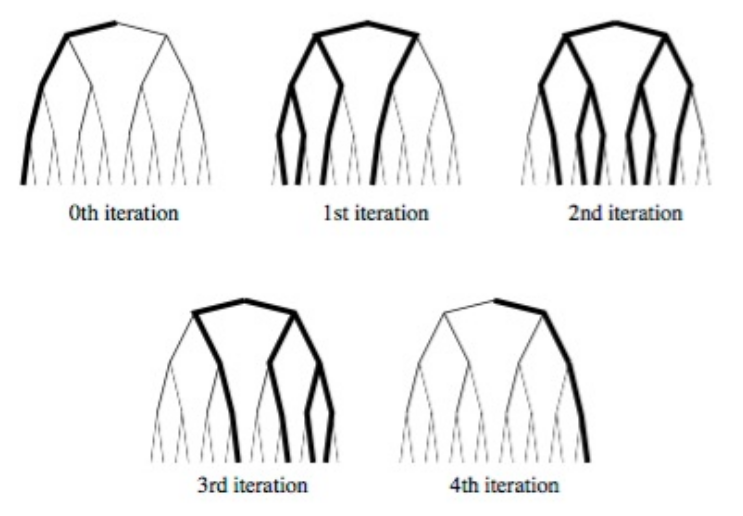
\includegraphics[scale=0.25]{lds.png}

\subsubsection{Depth-bounded discrepancy search}
Since it is more convenient to perform discrepancy at the highest levels of the
tree instead of the deepest ones, the discrepancy performing is done a bit
different from LDS: at the i-th iteration, discrepancy branches are visited only
if they are at the i-th level, otherwise the original heuristic is followed.

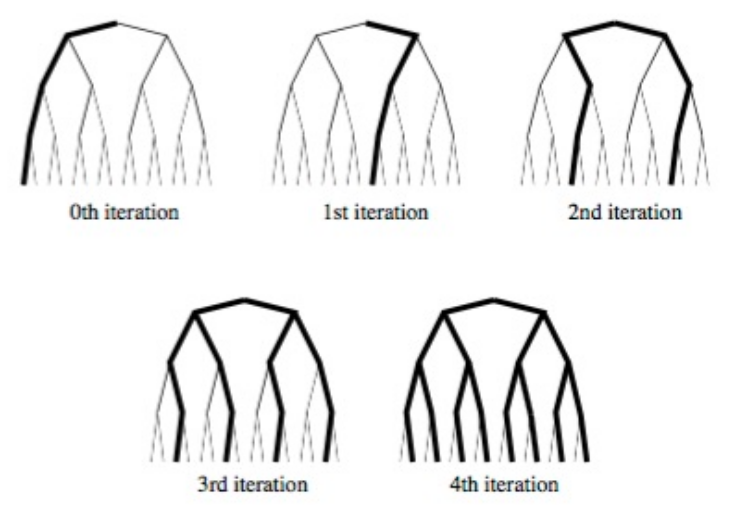
\includegraphics[scale=0.25]{dds.png}

The problem with LDS is that it acts on the deepest branches, but often it is
useful to make different decisions at the highest levels because the search is
less informative and the bad decisions are likely to be taken tehre. DDS is
better than LDS from this point of view.

\subsection{Optimization problems}
An optimization problem is a 4-tuple $\langle X, D, C, f \rangle$ where $X$,
$D$ and $C$ are the decision variables, domains of variables and constraints
respectively while $f$ is an optimization criterion in the form of an objective
function. For example we can set the goal of a problem as the $min f$, so
minimizing the value of $f$ (remember that $f$ is a variable, not a function).
Another way to set the goal can be:

\begin{itemize}
    \item defining $f = max(X)$;
    \item defining the goal as the $min f$.
\end{itemize}
In this way, we are searching the minimum number of $f$ value such that it is
useful to solve a certain problem.

\paragraph{Destructive lower bound}
A possible technique to solve minimization (or maximization or stuff like those)
can be searching ``through the domain of f", namely try assigning values to $f$
at each iteration starting from the minimum of $D(f)$ until we reach a solution.
At each iteration, the value is increased. Is is named ``destructive" because
intermediate results are discarded. The solution is proved to be optimal.
Disadvantages for this algorithm are: if resources of search are limited,
then it's not granted that it finds a solution; it performs small steps (just
one). An advantage is that it makes constraints tighter at each iteration, so
propagation is helped. Another advantage is that it provides lower bounds.

\paragraph{Destructive upper bound}
It is the same mechanism of DLB, but it starts with $max D(f)$. However, when we
find a solution, it isn't proved that it is the optimal one, so we continue to
decrease values and search solutions. When we arrive at the case where it fails
to find the solution, then the previous iteration of the current case is proven
to be the optimal solution. The pros and cons of this algorithm are exactly
complementary to DLB.

\paragraph{Binary search}
The main idea is to consider upper bound and lower bound in an array (the
solutions domain). At each iteration, these bounds are restricted and come
closer in this way:
\begin{itemize}
    \item we set $lb < f < (lb + ub / 2)$, where $lb$ is lower bound and $ub$ is
    upper bound;
    \item we try to solve the problem for that value of $f$;
    \item if the problem is feasible, then we update $ub$, else we update $lb$;
    \item we repeat these procedures until we reach $f = lb + 1$, which is the
    optimal solution.
\end{itemize}
It takes advantages from both DLB and DUB. But it's not the best way, because
all information is discarded at each iteration, so we are performing duplicated
work.

\paragraph{Branch and bound}
It uses a single search tree, incorporating bounds in the search. At each
iteration, when a solution is found, a new bound constraint is set to ensure the
future solutions are better, then it backtracks and looks for a new solution.
This is repeated until the problem is infeasible, at that point, the last
solution is demonstrated to be optimal.

\section{Scheduling}
It concerns with ordering resources and/or tasks over time and it has a lot of
applications. We have:
\begin{itemize}
    \item a set of resources with fixed capacities;
    \item a set of tasks with durations and resource requirements;
    \item a set of temporal constraints, for example we may want task 1 to run
    before or after task 2;
    \item a performance metric, namely something to measure the goodness
    (usually the objective variable).
\end{itemize}

In this kind of problem, usually, we have to decide when tasks have to start.
The decision variables correspond to the operations/activities to be performed.
An activity $a_i$ has: a starting time $s_i$, a duration $d_i$ and an ending
time $e_i$. We will refer to the earliest start time as $EST_i$, to the latest
start time as $LST_i$, to the earliest end time as $EET_i$ and to latest end
time $LET_i$. Note that $EST_i$, $EET_i$, $LST_i$ and $LET_i$ (the latter called
deadline) correspond to the possible earliest or latest times (not necessarily
the real ones). There are two types of activity:
\begin{itemize}
    \item preemptive activities, which can be interrupted any time, and it holds
    $s_i + d_i \leq e_i $
    \item non-preemtpive activities, which cannot be interrupted by external
    agents and it holds $s_i + d_i = e_i $.
\end{itemize}

A resource is something available and limited for tasks to run. We have:
\begin{description}
    \item[cumulative/parallel] resources which allow multiple activities to run
    at the same time, for example, they can be a multi-core CPU. Formally, a
    resource $r_k$ is associated to a capacity $c_k$. Each activity $a_i$ has
    requirements $rq_{ik} \geq 0$ on resource $r_k$. Clearly, it must hold
    $rq_{ik} \leq c_k$. We have cumulative constraint which handles the resource
    requirements for activities;
    \item[unary/disjunctive/sequential] resources which allow activities to
    execute only one at a time regardless the resource capacity. The disjunctive
    constraint handles this type of resources.
\end{description}

\subsubsection{Temporal constraints}
Temporal constraints can model the fact some actvities must come before or after
other activities. But they can be finer: they can define \textit{time-legs},
namely they bound the difference between the end time and the start time of two
activities; they can define also \textit{time-windows}, namely pretending one or
more activities runs in a certain time window.

\subsubsection{Cost function}
We define \textit{makespan} as the completion time of the last activity.
The RCPSP (cumulative resources) and job shop (disjunctive resources) scheduling
cost functions are makespan and the objective is usually to minimize the
makespan. A makespan can be modeled in different ways, for example introducing
a dummy activity with duration 0 and that must run as the last activity or
taking the maximum of the starting times of activities plus their durations
(obtaining the ending times).

\subsection{RCPSP}
Take a look at a sample for RCPSP:
\begin{itemize}
    \item a project graph $\langle A, E \rangle$, where $A$ is the set of
    activities and $E$ are their ending time;
    \item a set $R$ of resource $r_k$ with a capacity $c_k$;
    \item each activity $a_i$ has a duration $d_i$ and a resource requirement
    $r_{ik}$
\end{itemize}
We can see activities as:

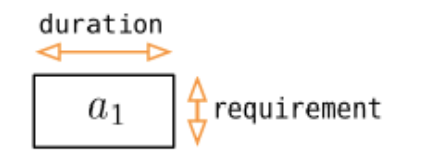
\includegraphics[scale=0.35]{activity.png}

\subsubsection{Search heuristics}
What are best heuristics for RCPSP? We must pose the following questions:
which variable to pick next? Which value to assign? Let's focus on the value
selection. Since the makespan has to be minimized, a good choice can be using
the minimum value (the $EST_i$). As far as variables choice is concerned, a good
choice can be selecting the one with the minimum $LET_i$. These are just
heuristics, so the optimal solution is not granted to be found immediately,
sometimes backtracking is necessary. Generally, since the objetive is to
minimize the makespan, increasing an $S_i$ cannot improve the makespan (we say
these problems have \textit{regular cost metrics}), so a good choice is the
$EST_i$ and this is true for many scheduling problems. But this is just a greedy
solution for a fast first solution, indeed, in order to reach optimality we have
to do backtracking. How to backtrack? Given a non-optimal solution, we select an
activity $a_i$ and instead of choosing the value for that variable, we postpone
it and we visit a subtree. Doing this procedure will grant optimality, but it's
often very expensive in terms of time. This technique regards both value and
variable choices.

And what about variable selection? Precedence constraints help us because they
make variables domains shrink. A good greedy choice can be selecting the task
with the minimum $LET_i$, so the one with the first deadline in order to discard
it immediately and to have the lowest probability for it to get a blind spot. To
reach optimality, refer to the technique explained before.

\section{Heuristic search}
We have two types of methods: complete methods, which guarantee the optimal
solution to each finite-size instance of a problem in a finite time; approximate
methods, which don't guarantee neither optimality, nor termination in case of
infeasibility, but they can find better solutions than complete methods in a
lower amount of time. We have three types approximate methods: constructive
heuristics, local search, metaheuristics.

\subsection{Constructive heuristics}
This is the fastest approximation and it consists in constructing the solution
from scratch by repeatedly extending the current partial assignment until a
solution is found or the stopping conditions are satisfied. An example can be
the greedy heuristics, but they don't guarantee optimality, but even though
this, they are quick and they are used as initialization step for other methods.

\subsection{Local search}
It gives often better solutions than constructive heuristics in terms of
optimality. It starts with an initial solution and it iteratively tries to
replace the current solution a with a better ``neighbourhood" (a near solution),
by applying small changes. Now we have to define what neighbourhood is, let's
see combinatorial optimization from a different perspective: given the problem
$\langle X, D, C, f \rangle$, $S$ the set of all solutions, we have to find
$s^* \in S$ such that $\forall s \in S. \; f(s^*) \leq f(s)$. We define a
function $N: S \mapsto \wp(S)$ that assigns to every $s \in S$ a set of
neighbours $N(s) \subseteq S$. $N(s)$ is called the \textit{neighbourhood} of
$s$. It is often implicitly defined by defining the modifications to $s$ to
reach $N(s)$. We now define a \textit{locally minimal solution} with respect to
a neighbourhood $N$ as a solution $s'$ such that
$\forall s \in N(s'). \; f(s') \leq f(s)$. A structure of local search algorithm
is done like this:
\begin{itemize}
    \item Generate a solution $s$;
    \item while $\exists s' \in N(s). \; f(s') \leq f(s)$, assign to $s$ an
    improving neighbor.
\end{itemize}
This algorithm stops when it finds a local minimum. There are different choices
of the neighbor: the first one or the best one. The first solution can be
generated randomly or heuristically. But how to define neighbourhood structure?
It comes useful the notion \textit{K-exchange neighbourhood}, where $K$ is the
number of modifications to do on the graph. In the problem of travelling
salesman problem, we can have that a starting solution is a hamiltonian tour
of the graph, then if we choose 2-exchange, we have to switch two archs, if
we choose 3-exchange, we have to switch three archs, etc.. Clearly, the more $K$
grows, the more neighbourhoods grows exponentially. Generally, a key issue is
how to define the neighbourhood. Too small neighbourhood is fast to find, but
the quality of local minima is low, while too large neighbourhood improves the
quality of local minima, but they are expensive to calculate.

\subsection{Metaheuristics}
They consist in higher level strategies which ``guide" heuristics to find a
solution. They can be seen, in simply terms, as heuristics on heuristics. We
have two types of policies: \textit{intensification} which exploits previous
experience; \textit{diversification} which explores the search space in the
large. A good balance between them is at the base of effectiveness of
metaheuristics.

\subsubsection{Local search methods}
It is similar to local search, but differently to it, this method tries to
escape to local minimum and it does it by allowing worsening solutions, by
changing neighbourhood structure during search or by changing objective function
during search. Clearly, we have to interrupt the algorithm at a certain point
since it cannot stop; some criteria are setting a maximum CPU time, number of
iterations, etc.. Here some methods.

\paragraph{Simulated annealing}
Like local search, but it accepts worsening moves with a certain probability.
The probability decreases at each iteration. It favours intensification over
diversification.

\paragraph{Variable neighbourhood search}
It changes neighbourhood structure during search, more precisely this happens
whenever a new local optima is reached.

\paragraph{Tabu search}
It keeps track of a ``tabu list" of solutions or moves and it forbids them. So
it doesn't change the neighbourhood, but it restricts the neighbors which it can
move to. Anyway, storing solutions is very inefficient, moves are cheaper even
if that could eliminate good solutions which haven't been visited yet. The tabu
list size is another important issue: the more it's big, the more
diversification grows against intensification. In general, the size can be
increased in case of repetitions (so when diversification is needed) or
decreased when there are no improvements (so intensification is needed).

\paragraph{Guided local search}
It changes the objective function. But one could argue it changes the semantics
of the claimed solution! The idea is to penalize some solution characteristics
which occur frequently, so the result is that some solutions get worse than how
they are really.

\subsubsection{Population-based methods}
We work on a set of solutions and the basic principle is to find common
characteristics among solutions. We have a probabilistic model from which we
obtain sample solutions to analyse. After this analysis, we update our model and
we restart the process. This process is similar to what ants do when they come
across an obstacle: the ants will try to find a path to escape from the
obstacle, then they will start to take the shortest path because it will be the
one which is walked by the majority of ants and the ants drop pheromones when
they walk and follow paths where the concentration of pheromones is higher. From
this phenomenon, we have the so-called \textit{pheromone model}: we have a set
of \textit{pheromone values} which act as the memory with the goal to focus the
search on certain paths. A way to make this concept formal can be: a
\textit{pheromone value} is a value $t(X_i, v_i)$, $\forall X_i \in X$ and
$v_i \in D(X_i)$ which represents the desirability of assigning $v_i$ to $X_i$.
A common usage is to have bounding for pheromone values $t_{min}$ and $t_{max}$
and to set initially values to $t_{max}$. As a consequence, we have that
decreasing values augment diversification because, we will have different values
from what we have had before (so it's like ants forget older solutions to get
close to newer solutions), while increasing will help intensification.

In order to begin, we use ``artificial ants". They simply consist in using
constructive heuristics for an initial solution. So the algorithm has the
following schema:
\begin{itemize}
    \item start from an initial solution, using constructive heuristics;
    \item iteratively choose a variable $X_i$ according to some heuristic (this
    is parametric) and then choose the value $v_i \in D(X_i)$ according to the
    probability:

    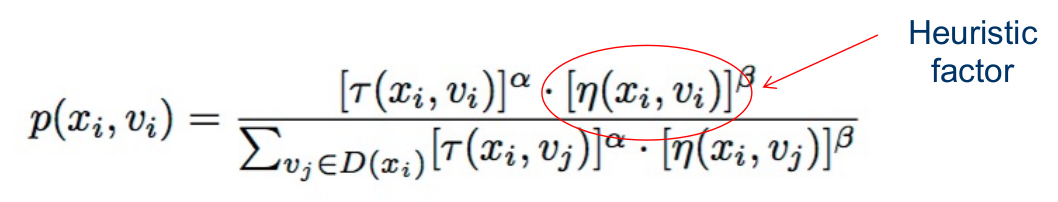
\includegraphics[scale=0.2]{prob_ants.png}    

    where $\alpha$ and $\beta$ are parameters used to balance the pheromone and
    heuristic factors.
\end{itemize}
Pheromone values in the $i$-th round are the ones which comes from $(i-1)$-th
round solutions. Then, at each round, pheromone values are updated. If they are
decreased, diversification is boosted, else if they are increased, then
intensification is boosted. The update is done in order to improve the quality
of future solutions.

At the end, which one to use? Local search metaheuristics or population-based
metaheuristics? It depends from the problem. If in the problem, moving from
neighbor to neighbor is easy and cheap in terms of computational cost, then
local search-based algorithms is good. On the other hand, if neighbourhood is
difficult to build, the cost of moves is not so cheap and solutions can be built
as composition of blocks, then population-based methods is a good idea.
Generally, local-based methods boost intensification because we act on subsets
of all solutions, while population-based methdos have the ability to boost
diversification (always according to how the pheromones are updated). Hybrid
methods tries to get the best from both methods types.

Metaheuristics is effective in finding first good-quality solutions, but it
struggles with complex constraints. For this reason, mixing metaheuristics and
complete methods in different ways can improve the quality of solutions in a
time unit, since complete methods, on the other hand, can be bad and inefficient
if we have loose bounds of objective function. For example, a complete method
can apply a metaheuristic to improve a solution or, on the contrary,
metaheuristics use a complete methods to efficiently to explore neighbourhood.

\paragraph{Large neighbourhood search}
And local search? How can it be combined with complete methods? Remember the
issue about small and large neighbourhoods; from this point, we can use large
neighbourhood and explore it with a complete method. We can see exploration of
neighbourhood as the solution of a sub-problem. So, given a solution $s$, we
have to possible moves to apply to each variable:
\begin{itemize}
    \item fix part of the variables value;
    \item relax the remaining variables.
\end{itemize}
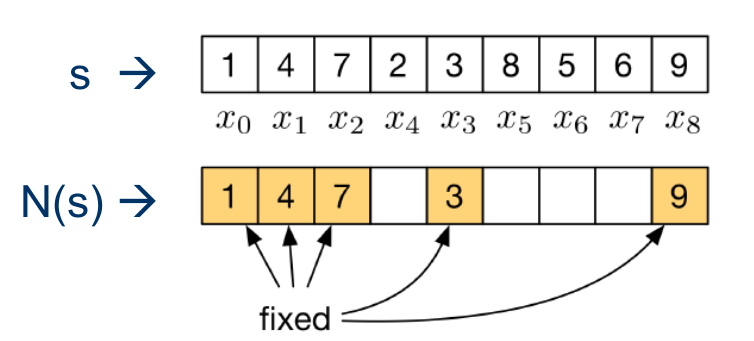
\includegraphics[scale=0.25]{fix_relax.png}

The good fact about this neighbourhood structure is that it works with all
problems. Now, two issues are: which percentage of variables to fix? Which
variables to fix? There are many ways to follow and it can depend from the
problem.

Generally, after wee saw all these different methods, the important thing is to
know how to mix these methods; to fix an optimization problem, the general good
way is to use a hybrid method.

\end{document}
